\documentclass{ccn}
% Bottom (and top) placement for double-column floats in \texttt{twocolumn} mode.
\usepackage{stfloats}
\addbibresource{ccn_references.bib}
\usepackage{booktabs}
\usepackage{bm}
% Coauthor fill-in markers; delete once text is finalized.
\newcommand{\TS}[1]{\textcolor{gray}{\footnotesize[TS: #1]}}

\title{Latent Dimensions of Interpretability in Visual Representations}

\author{%
  Author One\affmark{1} \And
  Author Two\affmark{1} \And
  Author Three\affmark{2} \And
  Author Four\affmark{2,3} \AND
  Author Five\affmark{3} \And
  Author Six\affmark{4} \And
  Author Seven\affmark{4} \And
  Author Eight\affmark{1,4}%
}
\affiliation{1}{Department of Neuroscience, First University}
\affiliation{2}{Institute for Brain Research, Second University}
\affiliation{3}{Center for Neural Computation, Third University}
\affiliation{4}{Department of Psychology, Fourth University}
\emails{author1@first.edu, author3@second.edu, corresponding@fourth.edu}


\begin{document}


\maketitle

% ORIGINAL ABSTRACT:
% What makes visual representations interpretable? In this work, we address this question by measuring the interpretability of visual features and examining how it relates to the alignment of models with properties of human perception, specifically human perceptual similarity. We find that models aligned with coarse—but not fine-grained—human similarity judgments tend to be more interpretable. Together, these results suggest that identifying properties of representations that promote interpretability provides a path toward making models systematically more interpretable to humans.

\begin{abstract}
  What makes the features learned by vision models interpretable to humans? We introduce a psychophysics protocol that directly measures feature interpretability—the degree to which a person, given a feature visualization and importance maps, can predict where that feature will activate in a new image. The logic is simple: if a feature captures a recognizable visual concept, observers should be able to localize it; if it does not, they will struggle. Applying this protocol to sparse autoencoder features from a range of vision transformers, we find that self-supervised and foundation models are consistently less interpretable than their supervised counterparts. While fine-grained alignment with human similarity judgments is uniformly high across models and does not predict interpretability, coarse-grained alignment—capturing semantic rather than perceptual structure—is a stronger correlate, suggesting that interpretability depends less on perceptual fidelity than on whether a model's representations reflect the semantic organization of human perception.
\end{abstract}

\begin{figure*}[!b]
  \centering
  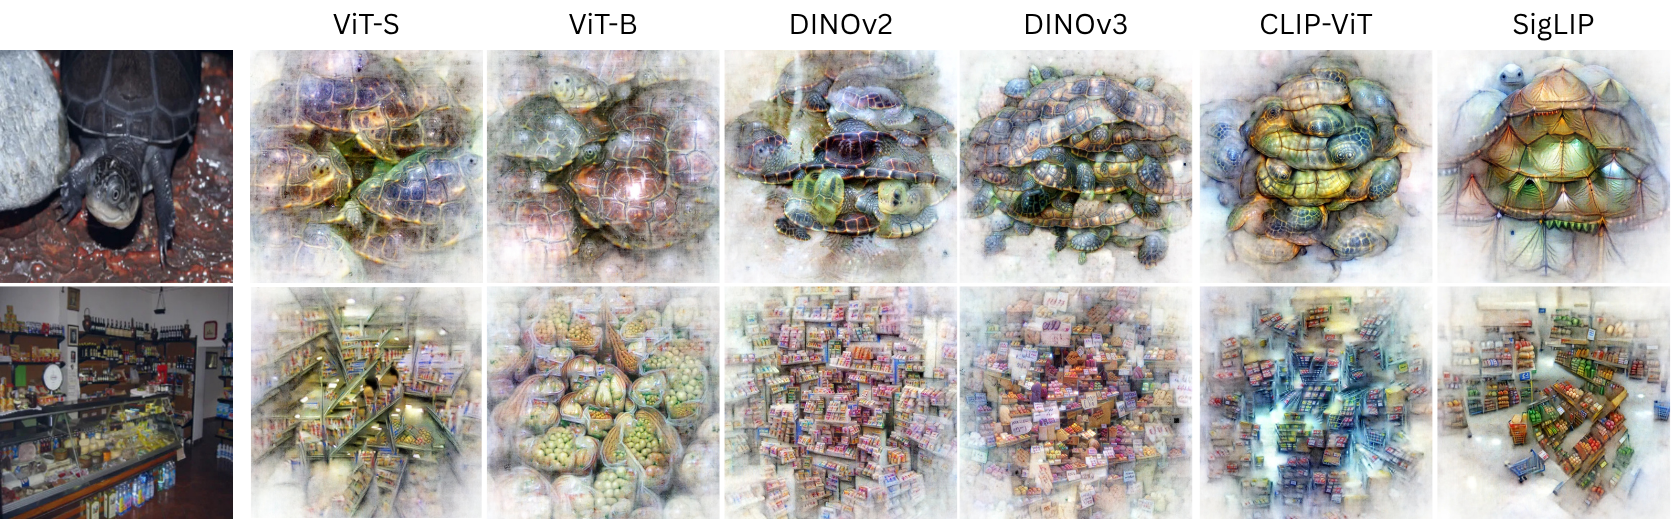
\includegraphics[width=0.88\textwidth]{Assets/features.png}
  \vskip -0.08in
  \caption{Most important feature for the prediction (top) \textit{mud turtle} and (bottom) \textit{grocery store}.}
  \label{features}
\end{figure*}


\section{Introduction}

% ORIGINAL P1:
% Understanding the internal representations of deep neural networks remains a major challenge, particularly in high-stakes domains such as medical applications, where trust in model predictions depends on understanding which features drive them. Despite growing interest in interpretability, it remains unclear what makes a representation easier for humans to understand.

A growing hope in the field is that aligning vision models with human perception will make them more interpretable. Yet this hypothesis remains largely untested: we lack both a rigorous measure of the interpretability of individual model features and a systematic comparison across models with varying degrees of human alignment. Here we address both gaps.

% ORIGINAL P2:
% A growing hope is that aligning models with human perception might make models more interpretable, but the impact of alignments on interpretability is still not well understood as there is a lack of human evaluation of the interpretability of models.

% ORIGINAL P3:
% In this work, we focus on representations and, more specifically, their visual features. We say that the visual feature of a model is interpretable to the extent that people can predict its location in new images. To operationalize this, we introduce a psychophysics protocol in which we explain a feature to participants and then ask them to localize it on novel images (Fig.~\ref{protocol}). This enables a direct and fine-grained assessment of human understanding of individual visual features.

We operationalize feature interpretability through a psychophysics protocol: participants are shown a feature visualization and importance maps, and asked to localize the feature on novel images (Fig.~\ref{protocol}). If a feature captures a recognizable visual concept, observers should be able to find it; if it does not, they will struggle. We apply this protocol to sparse autoencoder features extracted from a diverse set of vision transformers trained under different learning frameworks.

% ORIGINAL P4-5:
% We apply this experimental protocol to a diverse set of vision transformers (ViT) and investigate how their interpretability relates to alignment with human perceptual similarity judgments.
% We find that foundation models are generally harder to interpret than their supervised counterpart. Importantly, models aligned with coarse—but not fine-grained—human similarity judgments exhibit higher interpretability

We find that foundation models are consistently less interpretable than their supervised counterparts. Critically, while fine-grained alignment with human similarity judgments does not predict interpretability, coarse-grained alignment does—suggesting that representations capturing the semantic structure of human perception yield features that are easier for people to understand.


\section{Methodology}

% ORIGINAL:
% \paragraph{Models} We use a range of vision transformer trained under different representation learning framework. Unless specified otherwise, we use the base variant of the architecture. The specific models considered are: ViT-small, ViT, DINOv2, DINOv3, CLIP-ViT, SigLIP.

\paragraph{Features and models} For each model, we train a sparse autoencoder (SAE) to decompose the activations of the last layer into a dictionary of \TS{Julien fill: number of latent features, e.g., ``$K = 4{,}096$ latent features''} individual features over the ImageNet training set. A linear probe is trained on top of the frozen representations to estimate feature importance. Figure~\ref{features} shows examples of extracted features for two representative classes. We evaluate a diverse set of vision transformers spanning supervised and self-supervised learning frameworks: \TS{Julien fill: complete list with architecture sizes, e.g., ``ViT-S/16, ViT-B/16 (supervised), DINOv2 ViT-B/14, DINOv3 ViT-B/14, CLIP ViT-B/16, and SigLIP ViT-B/16''}. All models and their interpretability scores are summarized in Table~\ref{tab:results}.

\paragraph{Psychophysics experiment} For a given visual feature, we illustrate it via (i) a synthetic visualization, (ii) highly activating images, and (iii) corresponding importance heatmaps, and we ask participants to indicate its location on a novel query image (Fig.~\ref{protocol}). We select a representative set of features by sampling one image per superordinate class of ImageNet and retaining the top-3 most important features per image for the prediction of the model on that image (1,677 trials/model).

\begin{figure}[ht]
  \centering
  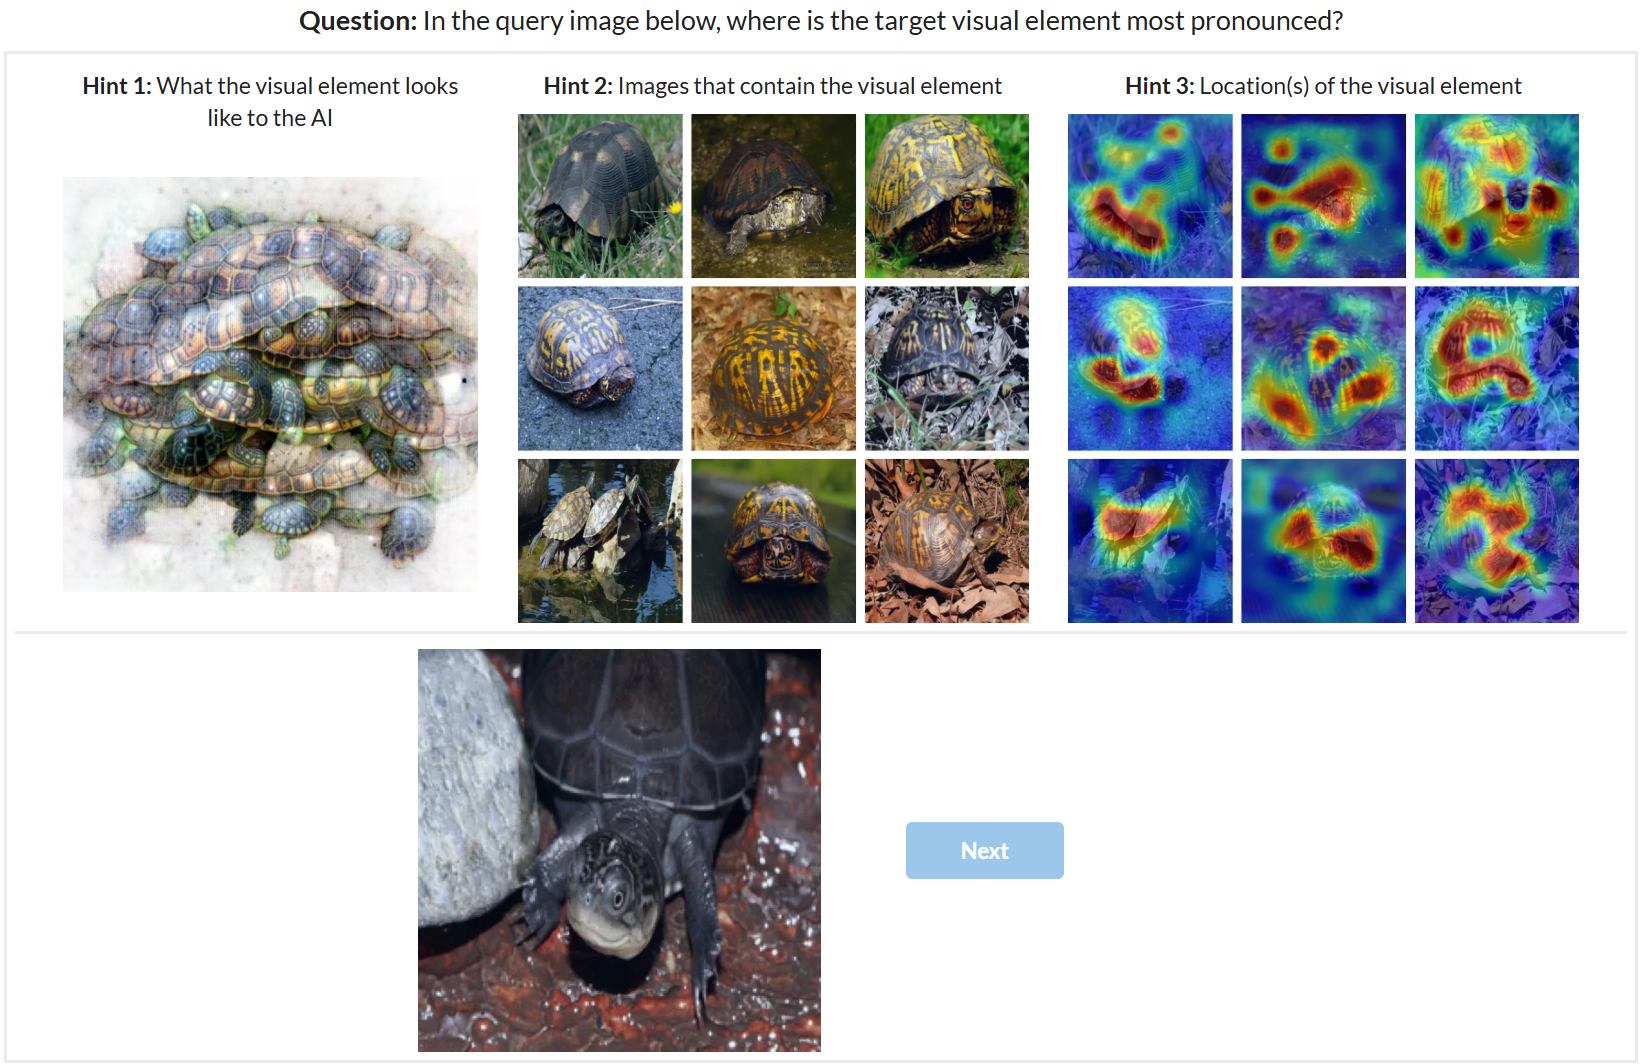
\includegraphics[width=\linewidth]{Assets/protocol.png}
  \caption{\textbf{Psychophysics experiment.} Example of a trial for DINOv3. The more interpretable the feature, the more likely participants are to correctly identify an area where the feature is present in the image.}
  \label{protocol}
\end{figure}

\paragraph{Interpretability score} Responses are scored using the empirical cumulative distribution function (ECDF) of the query heatmap value at the clicked location, measuring how strongly the selected region aligns with the feature relative to all possible locations in the image:
%
\begin{equation}
  \widehat{F}(v)
    \;=\;
    \frac{1}{n}
    \sum_{i=1}^{n}
    \mathbf{1}\!\left(x_i \le v\right),
\end{equation}
%
where $n$ is the number of pixels and $x_i$ denotes the degree to which the location $i$ contributes to the activation of the feature.

\paragraph{Alignment}
Human perceptual similarity is commonly measured with an odd-one-out task in which participants choose the least similar image from a triplet. The granularity of the resulting judgments depends on how the triplets are constructed. We leverage two complementary datasets: the THINGS odd-one-out dataset from Hebart et al.\ for coarse-grained similarity judgments, and the NIGHTS dataset for fine-grained similarity judgments. For each model, we measure alignment as agreement with human responses and relate it to the model's interpretability score.


\section{Discussion}


\begin{table}[h]
\caption{Interpretability results.}
\label{tab:results}
\vskip 0.05in
\centering
\footnotesize
\setlength{\tabcolsep}{3pt}
\resizebox{\columnwidth}{!}{
\begin{tabular}{lcccccc}
\toprule
 & ViT-S & ViT & DINOv2 & DINOv3 & CLIP-ViT & SigLIP \\
\midrule
Interpretability $\uparrow$  & 79.6 & \bm{85.9} & 70.4 & \underline{78.2} & 78 & 70.8 \\
Fine-grained Alignment $\uparrow$  & 85.2 & 83.9 & \underline{86.8} & \bm{87.8} & 83.5 & 85.1 \\
Coarse-grained Alignment $\uparrow$  & 47.5 & \underline{50.6} & 41.9 & 43.3 & \bm{50.7} & 40.8 \\
\bottomrule
\multicolumn{7}{l}{\scriptsize All values in \%. \textbf{Bold}: best. \underline{Underline}: second best.}
\end{tabular}
}
\end{table}

Increasing model capacity can help: ViT-B is more interpretable than ViT-S. More strikingly, self-supervised models (DINOv2, DINOv3) and vision-language models (CLIP, SigLIP) are consistently less interpretable than their supervised counterparts, despite comparable or superior classification accuracy. Indeed, classification performance on ImageNet~\cite{imagenet_cvpr09} is not correlated with interpretability ($r$=X, $p$=P).

Turning to alignment, fine-grained similarity scores are uniformly high across all models (83--88\%) and show no relationship with interpretability. Coarse-grained alignment, by contrast, is positively correlated with interpretability, consistent with the idea that features become more interpretable when a model's representations capture the semantic structure of human perception.


\section{Conclusion}
Our results provide direct evidence that aligning models with human perception—specifically at a semantic, coarse-grained level—is a promising route toward more interpretable vision models. Interpretability is often framed along two complementary axes: \emph{where} a feature activates and \emph{what} it represents. Here we have focused on the where; evaluating the complementary what is a natural next step toward a fuller picture of what makes representations interpretable.


\printbibliography

\end{document}
